%!TEX root = ../thesis.tex
%%%%%%%%%%%%%%%%%%%%%%%%%%%%%%%%%%%%%%%%%%%%%%%%%%%%%%%%%%%%%%%%%%%%%%%
%
% N=4 Super-Yang-Mills Theory
%
%%%%%%%%%%%%%%%%%%%%%%%%%%%%%%%%%%%%%%%%%%%%%%%%%%%%%%%%%%%%%%%%%%%%%%%
\chapter{Project Management}%
\chaptermark{Project Management}%
\label{chapter:project_management}

\section{Software Development Schedule}
\textbf{During the first month my focus will be on research, exploring various cloud-based technologies, comparing them, 
testing them and finalising the cloud service provider.}

\begin{figure}[!hb]
\centering
\caption[June Plan]{June Plan}%
\label{fig:june}
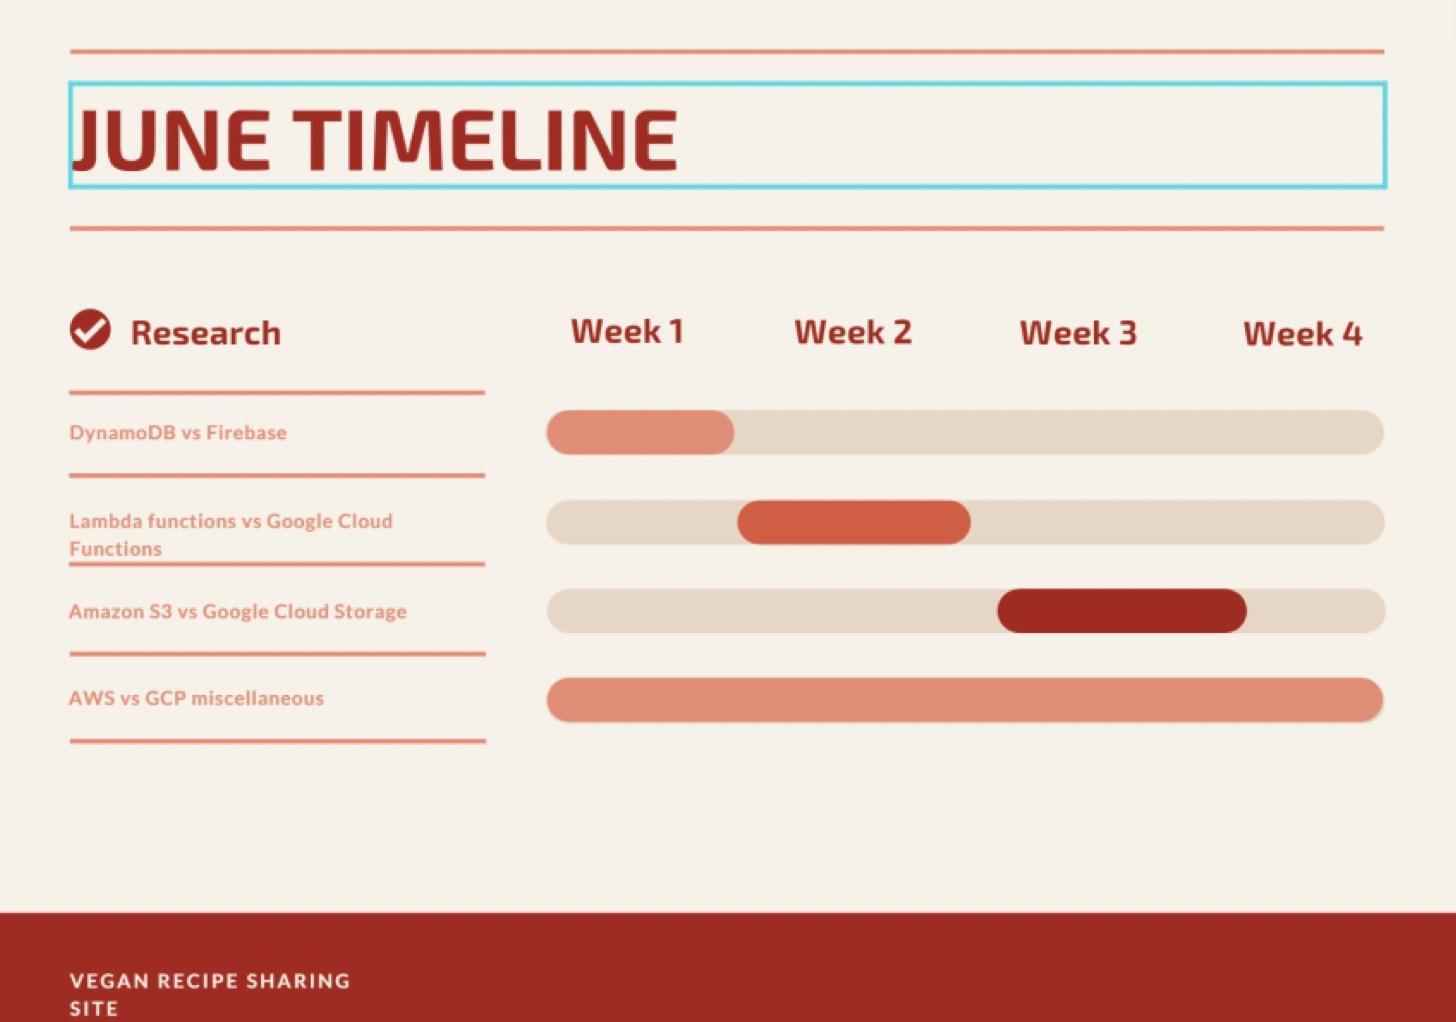
\includegraphics[width=\linewidth,height=\textheight,keepaspectratio]{img/june}
\end{figure}

\clearpage

\textbf{During the second month, I would be focusing on the front end, various frameworks, the best fit for my application 
and starting to build a User Interface.}

\begin{figure}[!hb]
\centering
\caption[July Plan]{July Plan}%
\label{fig:july}
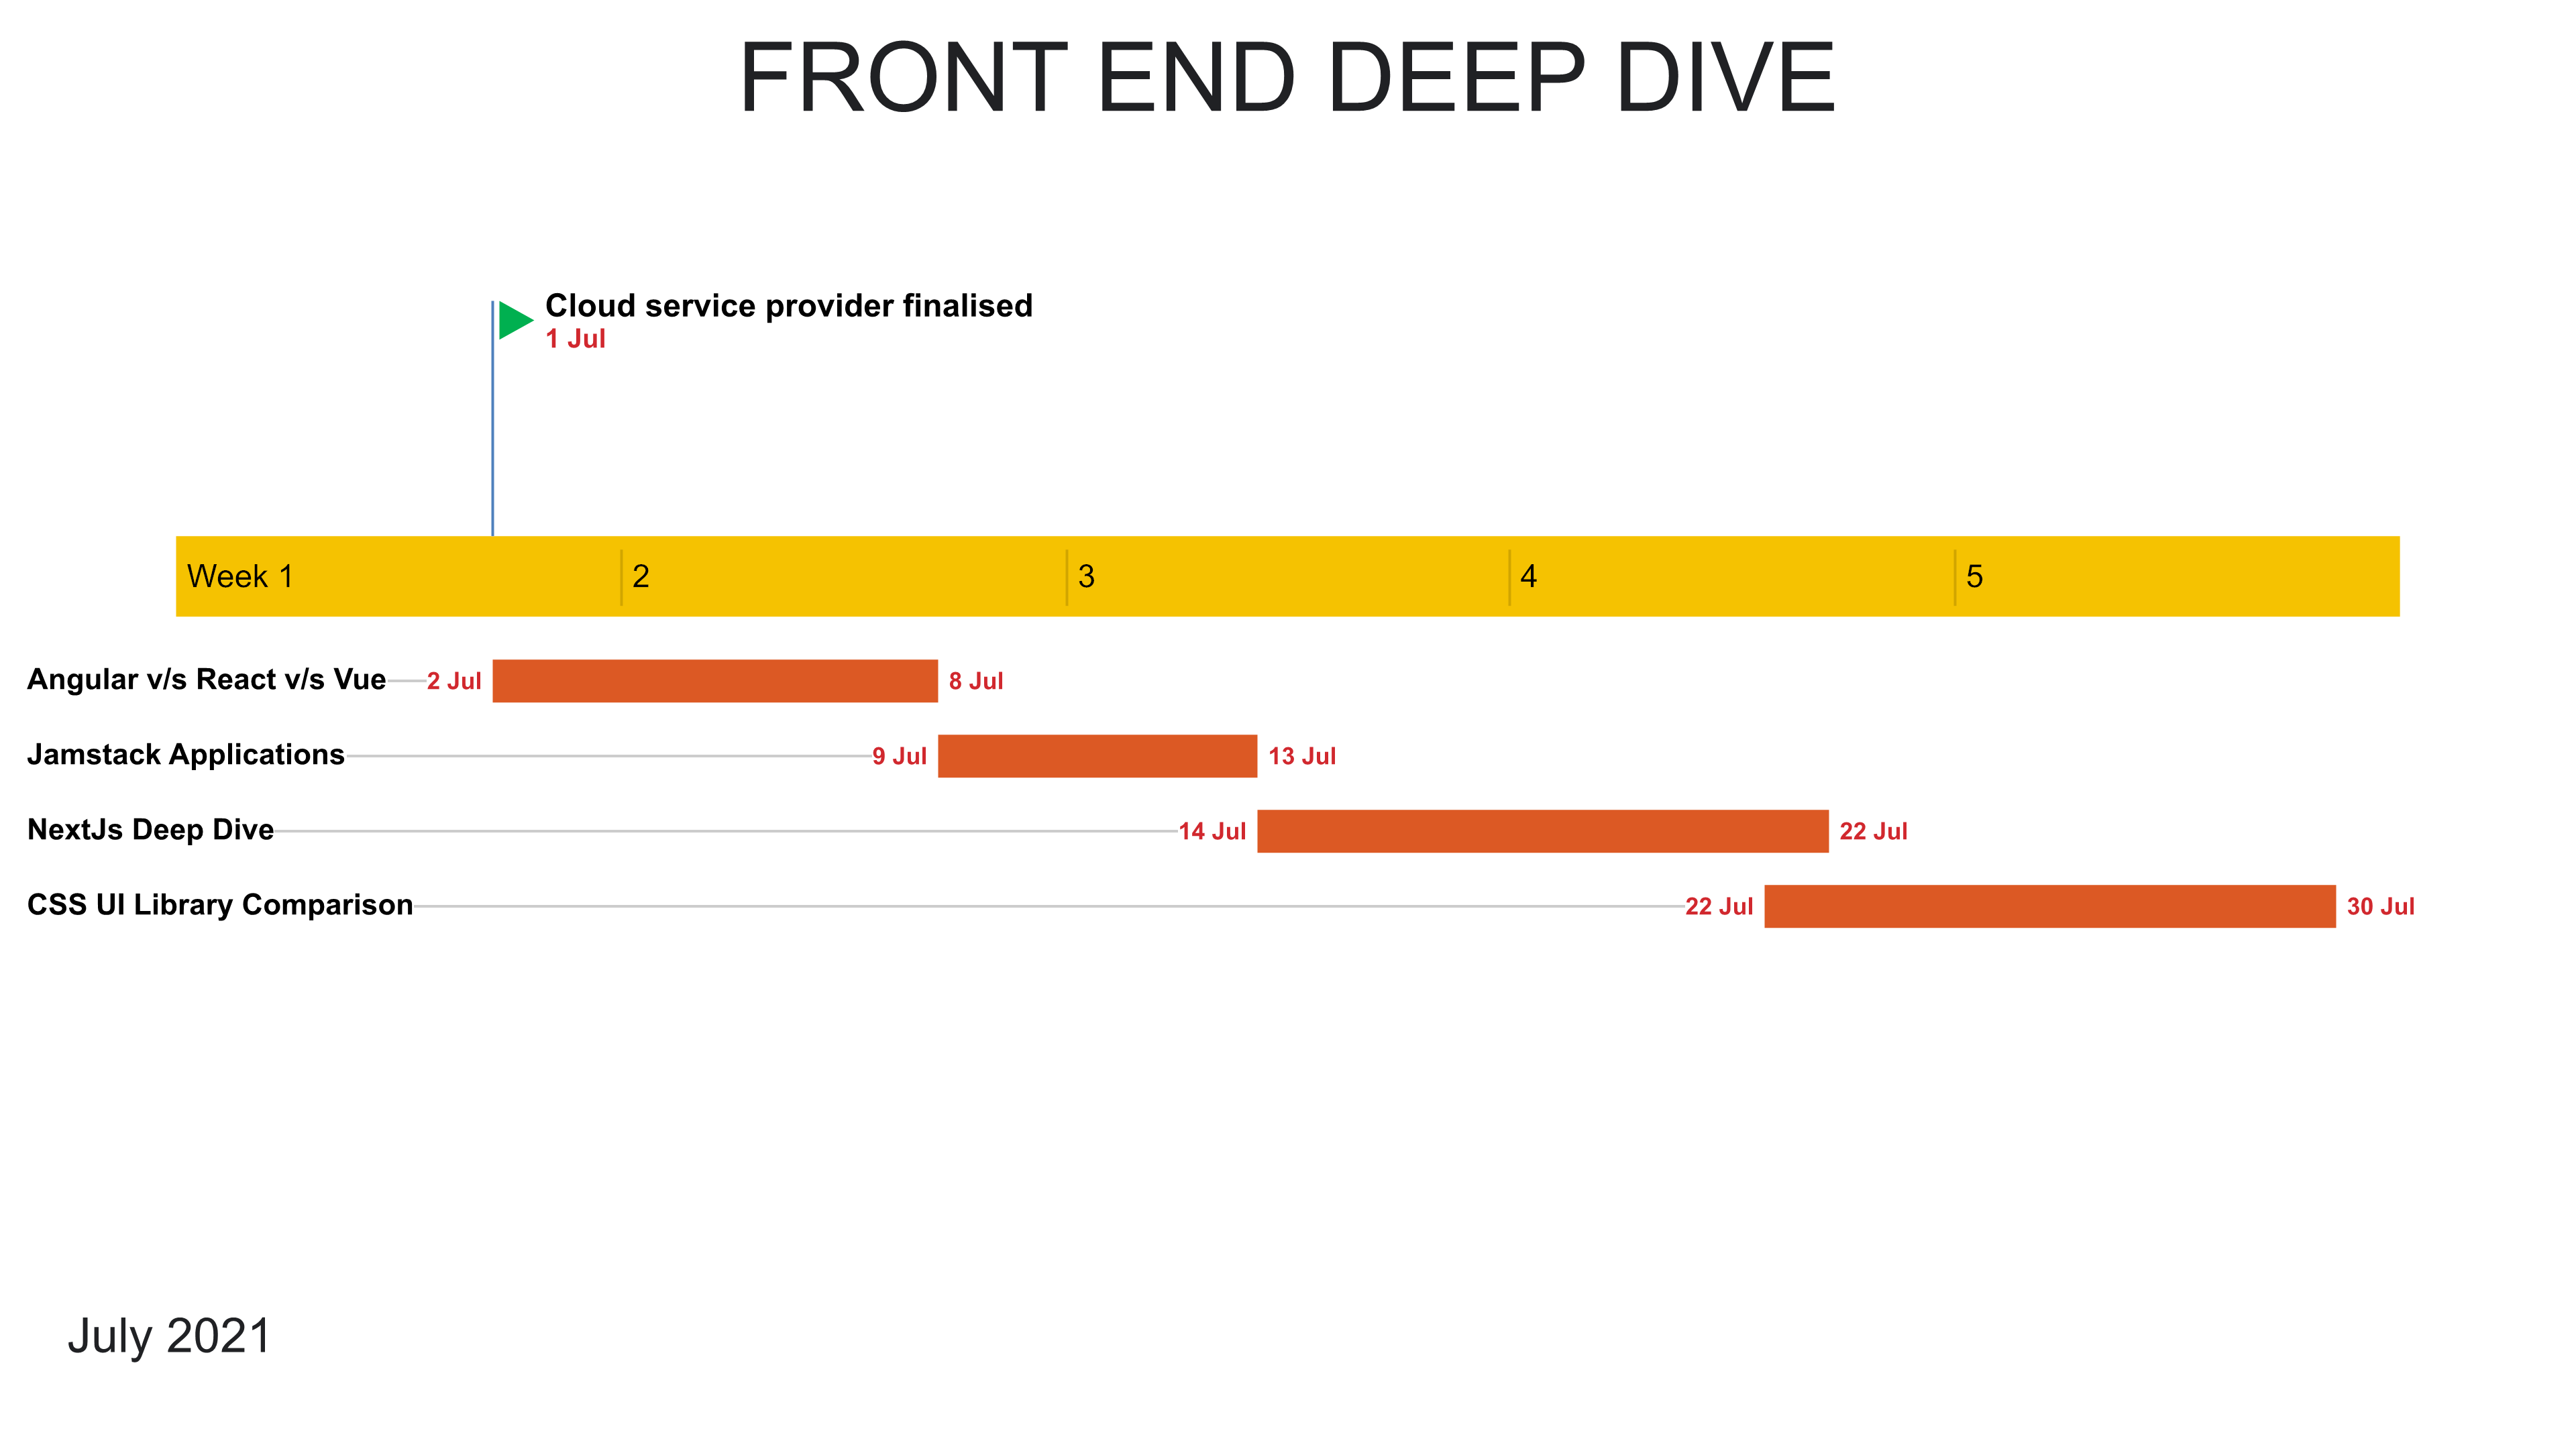
\includegraphics[width=\linewidth,height=\textheight,keepaspectratio]{img/july}
\end{figure}

\clearpage

\textbf{During the last month, I plan to work on the serverless backend, and its integration with the front end, 
to be ready with the final product.}

\begin{figure}[!hb]
\centering
\caption[August Plan]{August Plan}%
\label{fig:august}
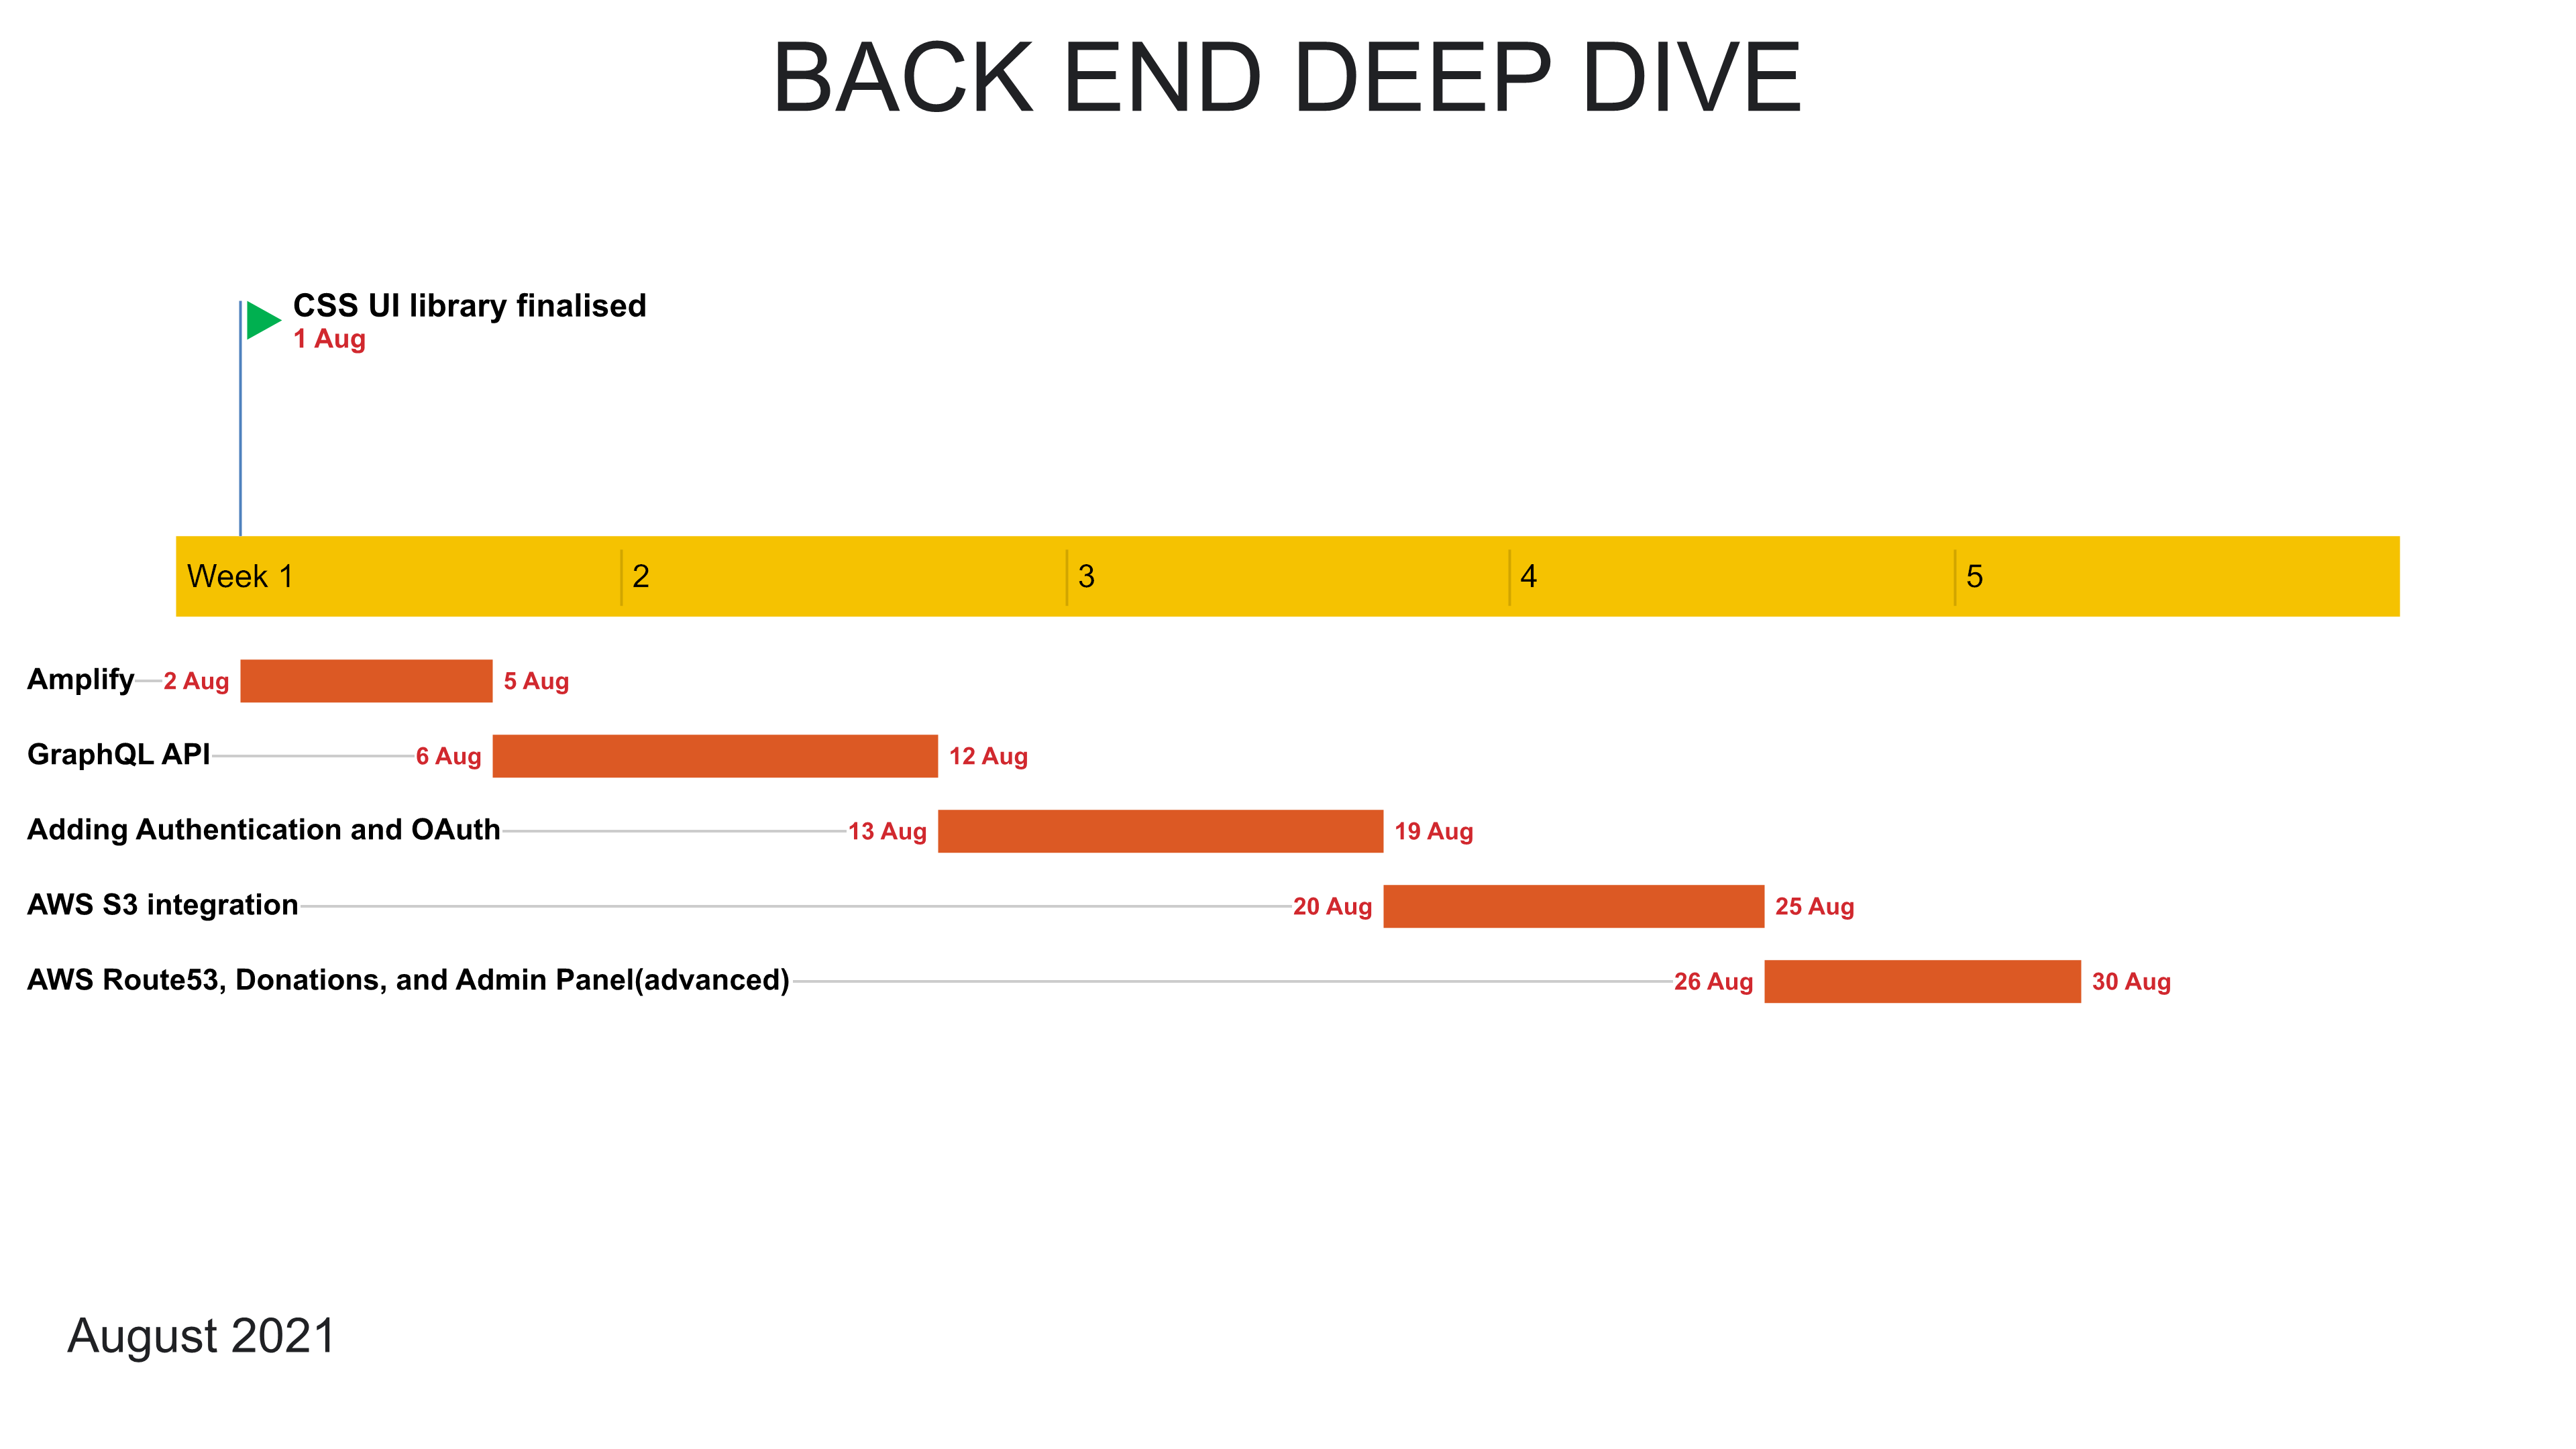
\includegraphics[width=\linewidth,height=\textheight,keepaspectratio]{img/august}
\end{figure}

\bigskip

\textbf{Some extra features I plan to work on are an admin dashboard, route53 as a DNS server and lambda functions for 
getting calories information via an API.}

\clearpage

\section{Software Development Methodology}

DevOps deployment methodology : DevOps is not just a development methodology but also a set of practices that supports an organizational culture. DevOps deployment centers on organizational change that enhances collaboration between the departments responsible for different segments of the development life cycle, such as development, quality assurance, and operations.

\bigskip

DevOps is focused on improving time to market, lowering the failure rate of new releases, shortening the lead time between fixes, and minimizing disruption while maximizing reliability. To achieve this, DevOps organizations aim to automate continuous deployment to ensure everything happens smoothly and reliably.

\bigskip

I aim to incorporate this methodology for the project, as it is one of the most popular models used in recent times, and is growing in popularity with effective CI/CD pipelines set up for deployment. As we use amplify for our project, our code is synced from github, our choice of version control, and changes we make are pulled into production.


\section{Risk Analysis}

In building a project of this scale, we are likely to have to account for certain risks and plan to mitigate them: 

\begin{itemize}
  \item External API dependency to nutritionix API, if they change the API format, our application will need updates. If their API stops working, an important calorie feature of our app will be missing.
  \item Updates in frontend libraries which we are using could make certain aspects obsolete, and would require a code review and refactor.
  \item Changes in the UI library which we are using to build certain components.
  \item Changes in the AWS features, like AppSync, lambda functions or even DynamoDB, while changes may not be breaking, could lead to depreciation and would cause maintenance issues.
  \item Domain name availability for our application depends on when we purchase and reserve the domain name from Route53.
\end{itemize}

While some of the risks mentioned are unavoidable, we could plan to mitigate a few. We can monitor the API and 
also shortlist some other backup services providing a similar functionality in case it goes down. Any updates on the 
frontend libraries, for example nextjs or ant design can be easily accommodated as we are following a DevOps deployment 
methodology, which fits our project well. All we need to do is make updates we need and push into github, and the changes 
will be easily integrated with our CI/CD pipeline. As for the domain name, we can purchase “theveganmanna” beforehand from 
route53 so that we do not have issues with availability. 


